
\chapter{آزمایشات و نتایج جدید}

در این فصل ما آزمایشات خود را مبنی بر پیاده سازی مدل هایی مبتنی بر معماری xLSTM برای ترمیم تصاویر ایستا بررسی و تفسیر می‌کنیم. مشاهداتی بر مدل سازی داده های غیرزمانی توسط معماری های زمانی مانند LSTM ارائه کرده و علل مد نظر خود را شرح و توجیه می‌کنیم.

\section{استفاده از LSTM و xLSTM در ترمیم تصویر}

در حالی که روش‌های سنتی و رویکردهای مدرن یادگیری عمیق مانند شبکه‌های عصبی پیچشی (CNN) و ترنسفورمرها موفقیت قابل توجهی نشان داده‌اند، شبکه‌های عصبی بازگشتی (RNN)، به‌ویژه شبکه‌های حافظه بلندمدت کوتاه‌مدت (LSTM)، برای این وظیفه کمتر مورد بررسی قرار گرفته‌اند. این کار به بررسی کاربرد معماری نوآورانه xLSTM در تکمیل تصویر یک‌تایی می‌پردازد و تمرکز آن بر روی جنبه‌های خروجی مدل است. ما به بررسی مبانی ریاضی، رفتار معماری و چالش‌هایی که در طول آزمایش‌ها با آن‌ها مواجه شدیم خواهیم پرداخت.

\subsection{معرفی مختصر LSTM}
شبکه‌های حافظه طولانی-کوتاه‌مدت (\lr{Long Short-Term Memory} یا \lr{LSTM})
\cite{hochreiterLongShortTermMemory1997}
، یک نوع خاص از شبکه‌های عصبی بازگشتی هستند که برای یادگیری وابستگی‌های بلندمدت در داده‌های دنباله‌ای طراحی شده‌اند. LSTM ها با استفاده از سلول‌های حافظه و مکانیزم‌های دروازه‌ای، مشکل فراموشی گرادیان که در شبکه‌های RNN سنتی رخ می‌دهد را کاهش می‌دهند. 

شبکه‌های عصبی بازگشتی بلند-کوتاه‌مدت (LSTM) از نظر ساختاری شباهت‌هایی به شبکه‌های عصبی بازگشتی استاندارد دارند، اما با این تفاوت که در اینجا هر گره بازگشتی معمولی با یک سلول حافظه جایگزین شده است. هر سلول حافظه شامل یک حالت داخلی است که به عنوان یک گره با اتصال بازگشتی خودکار و وزن ثابت 1 عمل می‌کند. این ویژگی منحصر به فرد باعث می‌شود که گرادیان‌ها بتوانند در طول گام‌های زمانی متعدد بدون مواجهه با مشکلاتی مانند ناپدید شدن (Vanishing) یا انفجار (Exploding) گرادیان، منتقل شوند. این مکانیسم به شبکه‌های LSTM امکان می‌دهد تا وابستگی‌های بلندمدت را در داده‌های متوالی به طور مؤثرتری یاد بگیرند و حفظ کنند.

\begin{figure}
	\centering
	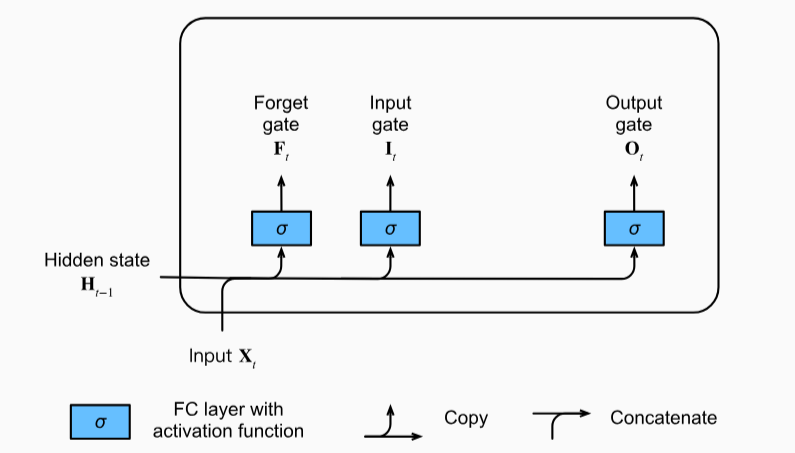
\includegraphics[width=0.7\linewidth]{lstm1}
	\caption{محاسبه گیت ورودی،‌ فراموشی و خروجی در یک سلول LSTM}
	\label{fig:lstm1}
\end{figure}

در مدل‌های شبکه‌های عصبی بازگشتی (RNN)، فرض کنید که تعداد واحدهای پنهان برابر با \( h \)، اندازه دسته برابر با \( n \) و تعداد ورودی‌ها برابر با \( d \) باشد. بنابراین، ورودی به شبکه در زمان گام \( t \) به صورت \( \mathbf{X}_t \in \mathbb{R}^{n \times d} \) و وضعیت پنهان گام زمانی قبلی به صورت \( \mathbf{H}_{t-1} \in \mathbb{R}^{n \times h} \) تعریف می‌شود. به طور مشابه، در هر زمان گام \( t \)، گیت‌ها به شرح زیر تعریف می‌شوند: گیت ورودی \( \mathbf{I}_t \in \mathbb{R}^{n \times h} \)، گیت فراموشی \( \mathbf{F}_t \in \mathbb{R}^{n \times h} \) و گیت خروجی \( \mathbf{O}_t \in \mathbb{R}^{n \times h} \). این گیت‌ها به صورت زیر محاسبه می‌شوند:

\[
\begin{aligned}
	\mathbf{I}_t &= \sigma(\mathbf{X}_t \mathbf{W}_{\textrm{xi}} + \mathbf{H}_{t-1} \mathbf{W}_{\textrm{hi}} + \mathbf{b}_\textrm{i}),\\
	\mathbf{F}_t &= \sigma(\mathbf{X}_t \mathbf{W}_{\textrm{xf}} + \mathbf{H}_{t-1} \mathbf{W}_{\textrm{hf}} + \mathbf{b}_\textrm{f}),\\
	\mathbf{O}_t &= \sigma(\mathbf{X}_t \mathbf{W}_{\textrm{xo}} + \mathbf{H}_{t-1} \mathbf{W}_{\textrm{ho}} + \mathbf{b}_\textrm{o}),
\end{aligned}
\]

که در آن \( \mathbf{W}_{\textrm{xi}}, \mathbf{W}_{\textrm{xf}}, \mathbf{W}_{\textrm{xo}} \in \mathbb{R}^{d \times h} \) و \( \mathbf{W}_{\textrm{hi}}, \mathbf{W}_{\textrm{hf}}, \mathbf{W}_{\textrm{ho}} \in \mathbb{R}^{h \times h} \) پارامترهای وزن هستند و \( \mathbf{b}_\textrm{i}, \mathbf{b}_\textrm{f}, \mathbf{b}_\textrm{o} \in \mathbb{R}^{1 \times h} \) پارامترهای بایاس هستند. در اینجا، از توابع سیگموید استفاده می‌شود تا مقادیر ورودی به بازه \( (0, 1) \) نگاشت شوند.


\subsection{جمع‌بندی}
اگرچه استفاده از LSTM و xLSTM برای ترمیم تصاویر به‌عنوان یک رویکرد نوآورانه مطرح شد، اما عدم وجود روابط زمانی در داده‌های تصویری و محدودیت‌های معماری شبکه‌های بازگشتی، کارایی این روش‌ها را محدود کرد. در نهایت، این مشاهدات نشان داد که ترکیب معماری‌های مبتنی بر توجه با سایر مکانیزم‌های بازنمایی مکانی، مانند Grid Embeddings، برای حل این مسئله ضروری است.

